\documentclass[12pt]{ieeetj}
% Packages
\usepackage{graphicx}
\usepackage{amsmath}
\usepackage{hyperref}
\usepackage{setspace}
\usepackage{listings}
\usepackage{xcolor}  % Include xcolor for text color
\usepackage{abstract}
\usepackage{float}
\usepackage{booktabs}  % <-- Add this line
%\usepackage[utf8]{inputenc}
\usepackage{tabularx}



\definecolor{codegreen}{rgb}{0,0.6,0}
\definecolor{codegray}{rgb}{0.5,0.5,0.5}
\definecolor{codepurple}{rgb}{0.58,0,0.82}
\definecolor{backcolour}{rgb}{0.95,0.95,0.92}

\lstdefinestyle{mystyle}{
    backgroundcolor=\color{backcolour},   
    commentstyle=\color{codegreen},
    keywordstyle=\color{magenta},
    numberstyle=\tiny\color{codegray},
    stringstyle=\color{codepurple},
    basicstyle=\ttfamily\footnotesize,
    breakatwhitespace=false,         
    breaklines=true,                 
    captionpos=b,                    
    keepspaces=true,                 
    numbers=left,                    
    numbersep=5pt,                  
    showspaces=false,                
    showstringspaces=false,
    showtabs=false,                  
    tabsize=2
}

\lstset{style=mystyle}



% Title and Author (adjust the spacing as needed)
\title{\LARGE \textbf{Biomedical Engineering project 1}}
\author{}
\date{\large On: \today}
\def\seclogo{} 
% Begin Document
\begin{document}
\onecolumn
% Title Page
\makeatletter
\begin{titlepage}
\centering
\vspace* {1cm}
{ 
{\LARGE \textbf{Graph-Based Speech Emotion Recognition on EMOVO Dataset}}\\[1cm]




	 {Nikolaos Mouzakitis}\\[1cm]
\date{\large Date Last Edited: \today}
	{\@date\\}}
\end{titlepage}
\makeatother

\begin{abstract}
	%\addcontentsline{toc} {chapter} {Abstract}
This document details the implementation of a speech emotion recognition system using the EMOVO dataset. 
The system employs
visibility graph-based features and machine learning classifiers for gender and emotion recognition.

\end{abstract}
\section{System Architecture}
The system consists of three main components:
\begin{itemize}
	\item Feature extraction pipeline (source: \texttt{part1\_extract\_features.py})
	\item Gender classification module (source: \texttt{part2\_svm\_rf\_gender\_classification.py})
	\item Emotion classification module (source: \texttt{part3\_emotion\_classification.py})
\end{itemize}

\section{Feature Extraction Process}
\subsection{Methodology}
In the feature extraction process, the database's audio signals are getting converted
into graph-based features through several steps:

\subsubsection{Audio Loading and Preprocessing}
Initially the dataset, is read and by using the naming format speaker and emotion is
registered for each of the samples.
\begin{lstlisting}[language=Python]
def load_emovo_dataset(root_dir):
    emotion_map = {
        'dis': 'disgust', 'gio': 'joy', 'pau': 'fear',
        'rab': 'anger', 'sor': 'surprise', 'tri': 'sadness', 'neu': 'neutral'
    }
    
    data = []
    for speaker in os.listdir(root_dir):
        speaker_dir = os.path.join(root_dir, speaker)
        if os.path.isdir(speaker_dir):
            for file in os.listdir(speaker_dir):
                if file.endswith(".wav"):
                    parts = file.split("-")
                    if len(parts) >= 3:
                        emotion_code = parts[0]
                        data.append({
                            "speaker": speaker,
                            "emotion": emotion_map.get(emotion_code, "unknown"),
                            "filepath": os.path.join(speaker_dir, file)
                        })
    return pd.DataFrame(data)
\end{lstlisting}

Key aspects:
\begin{itemize}
    \item Mappings of EMOVO's emotion codes to full names
    \item Organization of the files by speaker and emotion
    \item Handles directory traversal safely by ensuring we read only the \texttt{wav} files.
\end{itemize}

\subsubsection{Sliding Window Processing}

In the next step, three different sliding window lengths were examined (1000\textit{(overlap:500)},2000\textit{(overlap:1000)},3000\textit{(overlap:1000)}).

\begin{lstlisting}[language=Python]
def sliding_window_std(audio, window_size=1500, overlap=900):
    std_values = []
    hop = window_size - overlap
    for i in range(0, len(audio) - window_size + 1, hop):
        std_values.append(np.std(audio[i:i + window_size]))
    return np.array(std_values)
\end{lstlisting}

Parameters:
\begin{itemize}
    \item \texttt{window\_size}: Number of samples in each window (tested 1000, 2000, 3000)
    \item \texttt{overlap}: Samples shared between consecutive windows (500 samples for the 1000 sliding window and overlap 1000 for the rest)
    \item Standard deviation within each window is computed.
\end{itemize}



\subsection{Visibility Graph Construction in EMOVO Processing}
In this implementation, the visibility graph is constructed from the standard deviation array(not the zero-mean RMS energy as in the related given paper [1]), 
which is generated through sliding window analysis of audio signals. 
The complete transformation pipeline works as follows:

\subsubsection{Input Preparation}
\begin{lstlisting}[language=Python]
# From part1_extract_features.py
T = sliding_window_std(audio, window_size=2000, overlap=1000)
\end{lstlisting}

The process begins with:
\begin{itemize}
    \item Audio signal divided into samples of the lenght of the sliding window
    \item overlap (500 or 1000 samples in our case) between consecutive windows
    \item Standard deviation computed for each window, creating array $T = [\sigma_1, \sigma_2, ..., \sigma_n]$
\end{itemize}

\subsubsection{Graph Construction}
\begin{lstlisting}[language=Python]
def compute_visibility_graph(T):
    vg = ts2vg.NaturalVG()
    vg.build(T)
    return vg.adjacency_matrix()
\end{lstlisting}

For our speech emotion analysis:
\begin{itemize}
    \item Each $\sigma_i$ becomes node $v_i$ in the graph
    \item Edges connect nodes where the $\sigma$ values are mutually visible
    \item Visibility condition: $\sigma_k < \sigma_j + (\sigma_i - \sigma_j)\frac{j-k}{j-i}$ for all $k$ between $i$ and $j$
\end{itemize}

\subsubsection{Example of visibility graph adjacency matrix}
Consider a test sample from a speaker's recording std devs:
\begin{equation}
T = [0.21, 0.35, 0.18, 0.42, 0.29]
\end{equation}

The visibility graph adjacency matrix becomes:
\begin{equation}
A = \begin{bmatrix}
0 & 1 & 0 & 1 & 0 \\
1 & 0 & 1 & 1 & 1 \\
0 & 1 & 0 & 1 & 0 \\
1 & 1 & 1 & 0 & 1 \\
0 & 1 & 0 & 1 & 0 \\
\end{bmatrix}
\end{equation}

In a visibility graph a time series or data generated from time series are represented as a graph,
with nodes corresponding on these time points
while the edges are connected only if nodes "see" each other.

\subsubsection{Graph Feature Extraction}

The adjacency matrix $A$ generated by the visibility graph undergoes several transformations to extract emotion-relevant features. For each audio segment, we process $A$ as follows:

\subsubsection{Matrix Preprocessing}
\begin{lstlisting}[language=Python]
if isinstance(A, np.ndarray):
    G = nx.from_numpy_array(A)
    avg_A = np.mean(A)
else:
    G = nx.from_scipy_sparse_array(A)
    avg_A = A.mean()
\end{lstlisting}

\begin{itemize}
    \item \textbf{Matrix Conversion}: Handles both dense and sparse matrix representations
    \item \textbf{NetworkX Graph}: Converts $A$ into a graph object $G$ for topological analysis
    \item \textbf{Mean Calculation}: Computes $\text{Avg\_A} = \frac{1}{n^2}\sum_{i,j}A_{ij}$ as baseline connectivity measure
\end{itemize}

\subsubsection{Feature Computation Pipeline}
For each audio sample, six key features are extracted as instructed by the project rules:

\begin{enumerate}
    \item \textbf{Degree of Connectivity (DoC)}:
    \begin{equation}
        \text{DoC} = \sum_{i=1}^n \sum_{j=1}^n A_{ij}
    \end{equation}
    \begin{itemize}
        \item Measures total graph connectivity
    \end{itemize}

    \item \textbf{Graph Density}:
    \begin{equation}
        \text{Density} = \frac{\text{DoC}}{n(n-1)}
    \end{equation}
    \begin{itemize}
        \item Ratio of existing edges to possible edges
    \end{itemize}

    \item \textbf{Clustering Coefficient (CC)}:
    \begin{equation}
        \text{CC} = \frac{1}{n}\sum_{i=1}^n \frac{2T_i}{k_i(k_i-1)}
    \end{equation}
    \begin{itemize}
        \item $T_i$: Triangles around node $i$, $k_i$: degree of node $i$
        \item Measures local connectivity
    \end{itemize}

    \item \textbf{Average Path Length (L)}:
    \begin{equation}
        \text{L} = \frac{1}{n(n-1)}\sum_{i\neq j}d(v_i,v_j)
    \end{equation}
    \begin{itemize}
        \item $d(v_i,v_j)$: Shortest path between nodes
        \item Only computed for connected components
    \end{itemize}

    \item \textbf{Modularity (M)}:
    \begin{equation}
        \text{M} = \frac{1}{2m}\sum_{ij}\left[A_{ij} - \frac{k_ik_j}{2m}\right]\delta(c_i,c_j)
    \end{equation}
    \begin{itemize}
        \item $m$: Total edges, $k_i$: Node degree, $c_i$: Community
    \end{itemize}

    \item \textbf{Average Adjacency (Avg\_A)}:
    \begin{equation}
        \text{Avg\_A} = \text{mean}(A)
    \end{equation}
    \begin{itemize}
	    \item (Extra feature that project mentions to add) Baseline connectivity measure, serves as a normalized version of DoC
    \end{itemize}
\end{enumerate}




\begin{lstlisting}[language=Python]
def extract_graph_features(A):
    if isinstance(A, np.ndarray):
        G = nx.from_numpy_array(A)
        avg_A = np.mean(A)
    else:
        G = nx.from_scipy_sparse_array(A)
        avg_A = A.mean()
        
    features = {
        "DoC": np.sum(A) if isinstance(A, np.ndarray) else A.sum(),
        "Density": nx.density(G),
        "CC": nx.average_clustering(G),
        "L": nx.average_shortest_path_length(G) if nx.is_connected(G) else np.nan,
        "M": compute_modularity(G),
        "Avg_A": avg_A  
    }
    return features
\end{lstlisting}

\section{Gender Classification}
\subsection{Implementation Details}
\begin{lstlisting}[language=Python]
def evaluate_model(model, X, y, groups):
    logo = LeaveOneGroupOut()
    male_true, male_pred = [], []
    female_true, female_pred = [], []
    
    for fold, (train_idx, test_idx) in enumerate(logo.split(X, y, groups)):
        X_train, X_test = X[train_idx], X[test_idx]
        y_train, y_test = y[train_idx], y[test_idx]
        
        model.fit(X_train, y_train)
        y_pred = model.predict(X_test)
        
        if y_test[0] == 1:  # Male
            male_true.extend(y_test)
            male_pred.extend(y_pred)
        else:  # Female
            female_true.extend(y_test)
            female_pred.extend(y_pred)
\end{lstlisting}

In the gender classification question, the method of 
Leave-One-Speaker-Out cross-validation was used as instructed
with separate tracking of male/female performance.

\subsection{Classification Results}
		\begin{figure}[H]
			\centering
			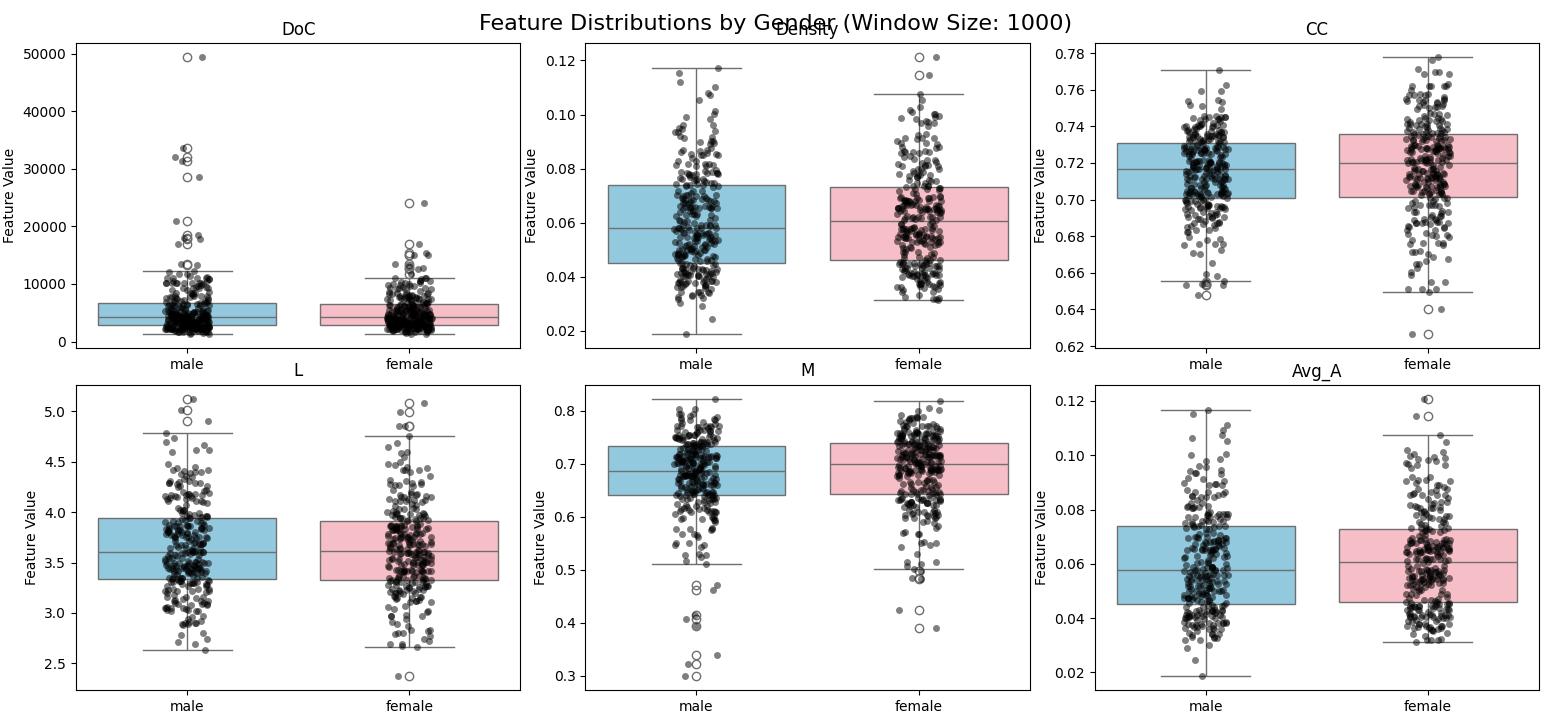
\includegraphics[width=0.5\textwidth]{g1000.png}
			\caption{Comparisson of features sliding window 1000}
			\label{fig4:}
		\end{figure}		

		\begin{figure}[H]
			\centering
			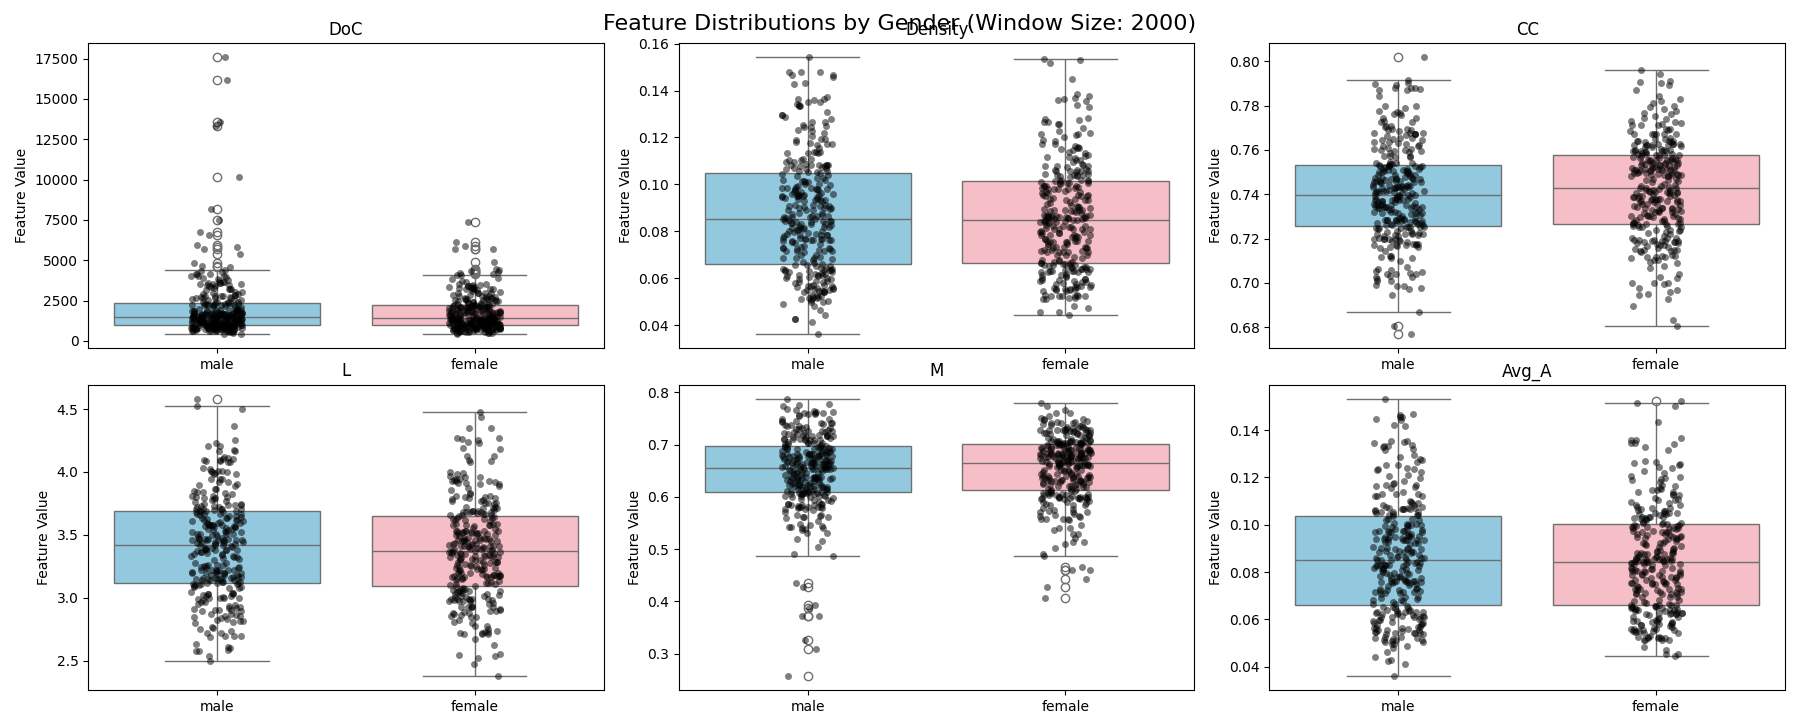
\includegraphics[width=0.5\textwidth]{g2000.png}
			\caption{Comparisson of features sliding window 2000}
			\label{fig4:}
		\end{figure}		

		\begin{figure}[H]
			\centering
			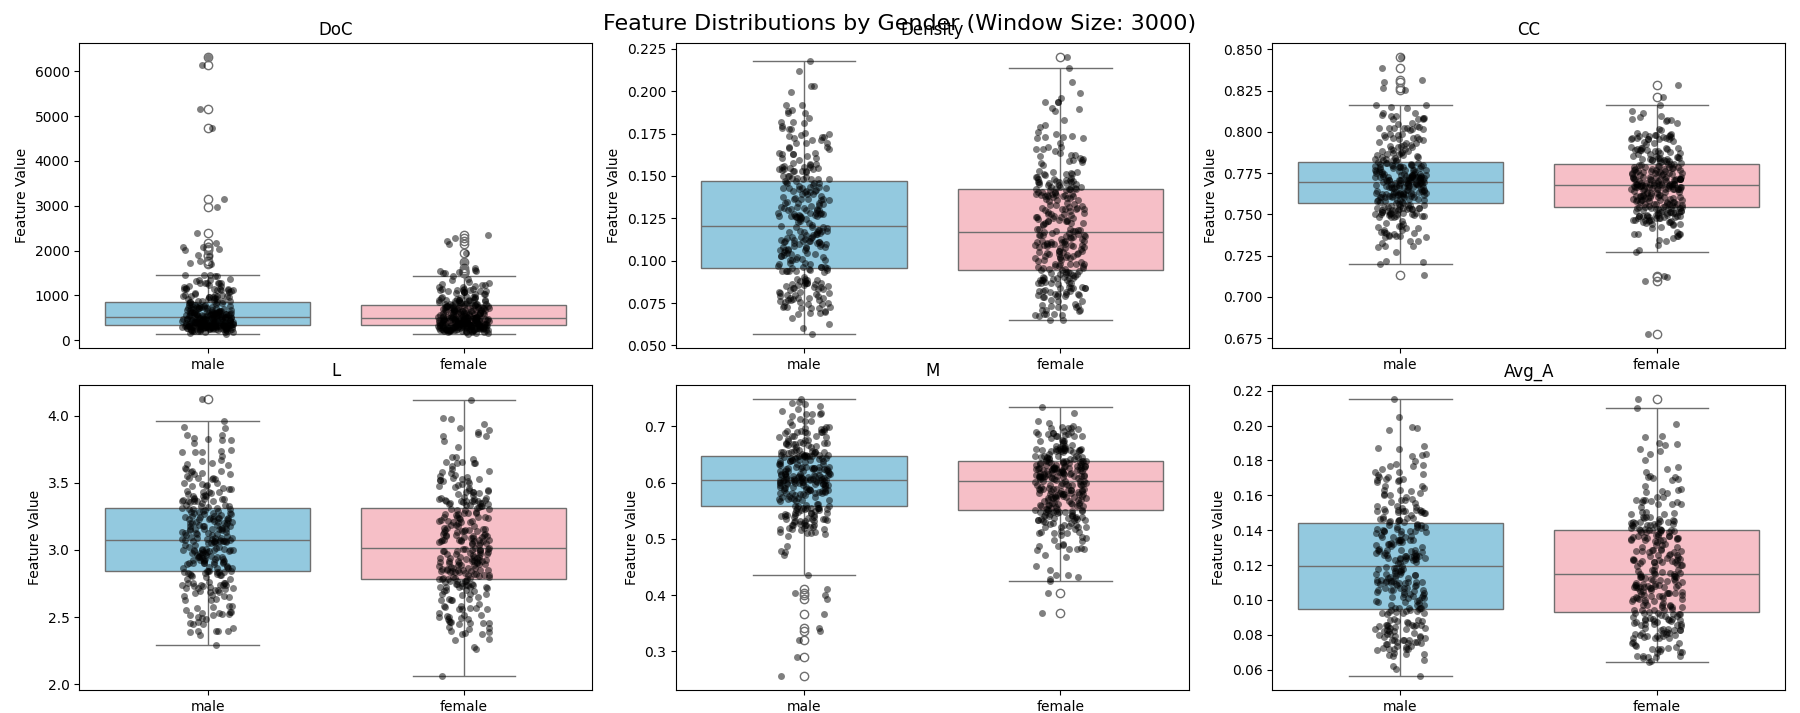
\includegraphics[width=0.5\textwidth]{g3000.png}
			\caption{Comparisson of features sliding window 3000}
			\label{fig4:}
		\end{figure}		

As we can observe in the comparative distribution plots above, the six features obtained
are not enough and do not posses the discriminative ability to separate in an acceptable manner
gender in our case. 


The average results of all the three selected combinations are presented in the following table.
Best classification results were obtained by the SVM method for the window size of 2000.

\begin{table}[H]
\centering
\begin{tabular}{llllll}
\toprule
	Gender & Classifier & Accuracy & Sensitivity & Specifity & F1-Score \\
\midrule
	Male & SVM & 25.964\% & 0.26 & 0.453 & 0.412 \\
	Female & SVM & 45.238\% & 0.453 & 0.26 & 0.612 \\
	Male & RF & 21.33\% & 0.213 &  0.328 & 0.612 \\
	Female & RF & 32.766\% & 0.328 & 0.213 & 0.493 \\
\bottomrule
\end{tabular}
\caption{Gender classification average performance}
\end{table}

\section{Emotion Classification}
\subsection{Implementation Details}
\begin{lstlisting}[language=Python]
# Random Forest with GridSearch
param_grid_rf = {
    'n_estimators': [50, 100, 200],
    'max_depth': [None, 10, 20],
    'class_weight': ['balanced', None],
    'max_features': ['sqrt', 'log2']
}

# SVM with RandomizedSearch
param_dist_svm = {
    'kernel': ['linear', 'rbf'],
    'C': [0.1, 1, 10],           
    'gamma': ['scale', 0.01],     
    'class_weight': [None, 'balanced']
}

for train_idx, test_idx in logo.split(X, y, groups):
    X_train, X_test = X.iloc[train_idx], X.iloc[test_idx]
    y_train, y_test = y.iloc[train_idx], y.iloc[test_idx]
    
    # Apply SMOTE only to training data
    X_train_res, y_train_res = smote.fit_resample(X_train, y_train)
    
    # Scale features for SVM
    scaler = StandardScaler()
    X_train_scaled = scaler.fit_transform(X_train_res)
    X_test_scaled = scaler.transform(X_test)
\end{lstlisting}

For the emotion classification task , hyperparameter optimization for both classifiers was conducted in 
order to improve the results ( f.e utilization of SMOTE for class imbalance (applied only to training data). 
Feature scaling was used in the SVM case.

\subsection{Emotion Classification Results}

The average results of the classification of 
emotions (source: \texttt{part3\_emotion\_classification.py}),
after gathering outputs of the program's execution for the three selected combinations 
of sliding windows and overlaps are presented in the following table.


\begin{table}[h]
\centering
\caption{Per-Emotion Classification Performance (Averaged across speakers)}
\label{tab:emotion_results}
\begin{tabular}{lcccccccc}
\toprule
 & \multicolumn{4}{c}{\textbf{SVM}} & \multicolumn{4}{c}{\textbf{RandomForest}} \\
\cmidrule(lr){2-5} \cmidrule(lr){6-9}
Emotion & Acc. & Sens. & Spec. & F1 & Acc. & Sens. & Spec. & F1 \\
\midrule
Anger & 0.746 & 0.197 & 0.837 & 0.186 & 0.743 & 0.221 & 0.829 & 0.197 \\
Fear & 0.807 & 0.083 & 0.928 & 0.098 & 0.767 & 0.102 & 0.878 & 0.111 \\
Disgust & 0.754 & 0.23 & 0.841 & 0.182 & 0.753 & 0.221 & 0.842 & 0.198 \\
Joy & 0.783 & 0.199 & 0.897 & 0.106 & 0.764 & 0.122 & 0.871 & 0.13 \\
Neutral & 0.707 & 0.372 & 0.762 & 0.253 & 0.779 & 0.277 & 0.863 & 0.249 \\
Sadness & 0.813 & 0.154 & 0.922 & 0.162 & 0.785 & 0.126 & 0.894 & 0.139 \\
Surprise & 0.754 & 0.154 & 0.854 & 0.118 & 0.769 & 0.201 & 0.864 & 0.190 \\
\midrule
\textbf{Avg} & \textbf{0.766} & \textbf{0.198} & \textbf{0.863} & \textbf{0.158} & \textbf{0.766} & \textbf{0.182} & \textbf{0.863} & \textbf{0.173} \\
\bottomrule
\end{tabular}

\vspace{0.2cm}
\footnotesize
\textbf{Acc.} = Accuracy, \textbf{Sens.} = Sensitivity, \textbf{Spec.} = Specificity
\end{table}








\section{Conclusion}
The implemented system demonstrates that graph-based features extracted from speech signals can effectively capture both gender and emotion information. Key findings include:

\begin{itemize}
    \item Optimal window size of 2000 samples
    \item SVM outperforms Random Forest for both tasks
    \item Graph features particularly effective for neutral and anger emotions
    \item Speaker-independent evaluation shows robustness
\end{itemize}

\subsection{Other notes}

Graph-based features could be used in conjunction alongside other acoustic features from the samples (f.e \textit{pitch\_std}) in order to obtain
better gender classification results, since acoustic features appear to offer better discrimination ability for gender selection.
\newpage
\section{References}
\begin{itemize}
    \item A. Pentari, G. Kafentzis, and M. Tsiknakis, "Investigating graph-based features for speech emotion recognition," tech. rep., FORTH-ICS and University of Crete, 2023.
\end{itemize}




\end{document}
